\documentclass[../main.tex]{subfiles}

\begin{document}

\chapter{计算机进阶}

我们在初阶课程中讲述的所谓“进阶”内容还是过于基础了,以至于无法称之为真正的“进阶”。因此,在本章中,我们将介绍一些计算机领域的进阶知识和技能,帮助同学们更深入地理解计算机的工作原理和应用。

\section{Git 进阶}\label{sec:git-advanced}

在初阶课程\ref{sec:git}中,我们已经介绍了 Git 的基本使用方法,包括如何创建仓库、提交代码、查看历史记录等。但是,Git 还有许多高级功能和技巧,可以帮助我们更高效地管理代码和协作。

\subsection{分支管理}

有时候我们想同时开发新功能,并且调优以前的代码,这样可能就需要两条线进行开发。这时,分支相关的功能就会很有帮助。Git 的分支功能允许我们在同一个仓库中创建多个独立的开发线,每个分支可以独立地进行提交和修改。

我们可以做如下假设:已经有一个名为main的分支,并已经有了一列提交记录A、B、C。现在,我希望开发一个新的功能,但是不想影响到main分支上的代码。这时,我们可以创建一个新的分支,例如feature,并在该分支上进行开发。

\subsubsection{创建和切换分支}

可以使用以下命令创建一个新的分支并切换到该分支:
\begin{lstlisting}[language=bash]
git checkout -b feature
\end{lstlisting}

以上等价于执行
\begin{lstlisting}[language=bash]
git branch feature <commit-hash of C>
git checkout feature
\end{lstlisting}

如果我现在想要回到main分支,可以使用以下命令:
\begin{lstlisting}[language=bash]
git checkout main
\end{lstlisting}

\subsubsection{分支变基}

如果我们已经在feature分支上进行了多次提交F、G,同时在main分支上也有了新的提交D、E。现在想要将feature这些提交变基到main分支上,可以使用以下命令:
\begin{lstlisting}[language=bash]
  git rebase main
  git checkout main
\end{lstlisting}
这样会把上述feature上的三个提交从C变基到E,变成F'和G'。我们可以用图解来理解这个过程:

\begin{figure}[htbp]
  \centering
  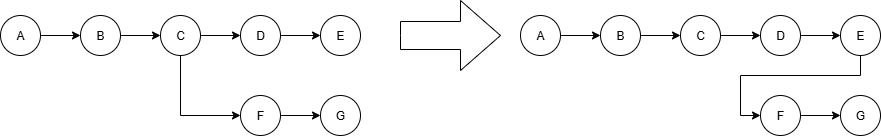
\includegraphics[width=\textwidth]{images/git-rebase.png}
  \caption{分支变基示意图}
  \label{fig:git-rebase}
\end{figure}

特别注意:变基操作会改变提交的哈希值。

\subsubsection{合并分支和冲突解决}

如果我们想要将feature分支上的代码合并(不是变基)到main分支上,可以使用以下命令:

\begin{lstlisting}[language=bash]
git checkout main
git merge feature
\end{lstlisting}

这时候我们在main分支上,并试图将E和G合并在一起。这时,会自动创建一个特殊的提交Merge,它有两个父提交。之后的提交就会以Merge为父提交,而不是E或G中的任何一个。

\begin{figure}[htbp]
  \centering
  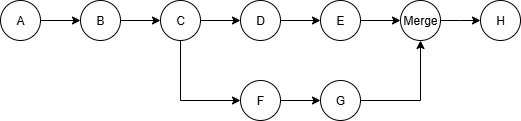
\includegraphics[width=0.75\textwidth]{images/git-merge.png}
  \caption{分支合并示意图}
  \label{fig:git-merge}
\end{figure}

如果这两个提交没有冲突,那么合并会自动完成。但是如果有冲突(例如两个分支涉及到同一行的修改),Git 会提示我们解决冲突。此时,我们不得不手动解决冲突。我们会看到以下内容(或者其英文版本):
\begin{lstlisting}[language=bash]
  自动合并 example1.txt
冲突(内容):合并冲突于 example1.txt
自动合并失败,修正冲突然后提交修正的结果。
\end{lstlisting}
此时,我们需要打开冲突的文件,手动解决冲突。Git 会在冲突的地方插入标记,例如:
\begin{lstlisting}[language=bash]
  <<<<<<< HEAD
  这是 main 分支上的内容。
  =======
  这是 feature 分支上的内容。
  >>>>>>> feature
\end{lstlisting}
我们需要手动编辑这个文件,删除这些标记,并保留我们想要的内容。

如果使用Code等编辑器,通常会有冲突解决的工具,可以帮助我们更方便地解决冲突。

解决完冲突后,我们需要使用以下命令来标记冲突已解决:
\begin{lstlisting}[language=bash]
  git add .
  git merge --continue
\end{lstlisting}

\subsubsection{删除分支}

如果我们已经完成了feature分支上的开发,并且已经将其合并到main分支上,可以使用以下命令删除该分支:
\begin{lstlisting}[language=bash]
git branch -d feature
\end{lstlisting}

一般不建议直接删除分支,而是使用 \texttt{-d} 选项来删除已经合并的分支。如果分支没有被合并,可以使用 \texttt{-D} 选项强制删除。

\subsubsection{压缩提交}

有时候,我们在开发过程中,可能会有很多小的提交,这些提交可能是一些临时的修改或者调试信息。为了保持代码和版本库的整洁,我们可以使用 Git 的压缩提交功能,将多个提交合并为一个提交。这个压缩功能被称作是\textbf{Squash},但是特别注意:没有\texttt{git squash}命令。

我们一般只在分支合并的时候使用压缩提交。可以使用以下命令中的一个来压缩提交:
\begin{lstlisting}[language=bash]
git merge --squash feature
\end{lstlisting}

\subsection{标签管理}
标签(Tag)是 Git 中用于标记特定提交的功能。标签通常用于标记版本发布或重要的里程碑。与分支不同,标签是静态的,不会随着提交而移动。

\subsubsection{创建标签}
可以使用以下命令创建一个标签:
\begin{lstlisting}[language=bash]
git tag v1.0
\end{lstlisting}

这将创建一个名为 v1.0 的标签,指向当前的提交。如果需要为特定的提交创建标签,可以在命令中指定提交的哈希值:
\begin{lstlisting}[language=bash]
git tag v1.0 <commit-hash>
\end{lstlisting}

\subsubsection{查看标签}
可以使用以下命令查看所有标签:
\begin{lstlisting}[language=bash]
git tag
\end{lstlisting}

\subsubsection{删除标签}
如果需要删除一个标签,可以使用以下命令:
\begin{lstlisting}[language=bash]
git tag -d v1.0
\end{lstlisting}

\subsection{“摘樱桃”}

Cherry-Pick(摘樱桃)操作(也叫挑拣)是指从一些提交中选择一些特定的提交(修改),并将这些提交(修改)应用到当前分支上。这适用于当我们只想要一些特定的提交而不是整个分支的所有提交的时候。

一般,CherryPick操作很难使用命令行来操作,其复杂程度过高。我们可以使用VS Code的自带Git视窗或者GitLens等工具来进行这个操作。

使用视窗进行挑拣非常方便,我们只需要在提交列表中选择需要的提交,然后右键点击“Cherry-Pick”(汉化应该是挑拣)即可。这样会将选中的提交应用到当前分支上。

\subsection{远程仓库}

很多项目无法只在一台机器上进行开发,往往都需要在远程部署一个仓库(例如GitHub、GitLab等,或者公司自建库),然后将本地的代码推送到远程仓库中。这样,我们就可以在不同的机器上从远程仓库中拉取代码,从而保证代码的一致性。

在本节,我们将使用 GitHub 作为远程仓库的示例,介绍如何将本地仓库与远程仓库进行关联、推送和拉取代码。

\subsubsection{创建仓库}
首先,我们需要在 GitHub 上创建一个新的仓库。创建完成后,GitHub 会提供一个远程仓库的 URL,例如:
\begin{lstlisting}
  https://github.com/YourName/example.git
\end{lstlisting}
我们可以在GitHub上的仓库页面中找到这个 URL,如图所示。

\begin{figure}[htbp]
  \centering
  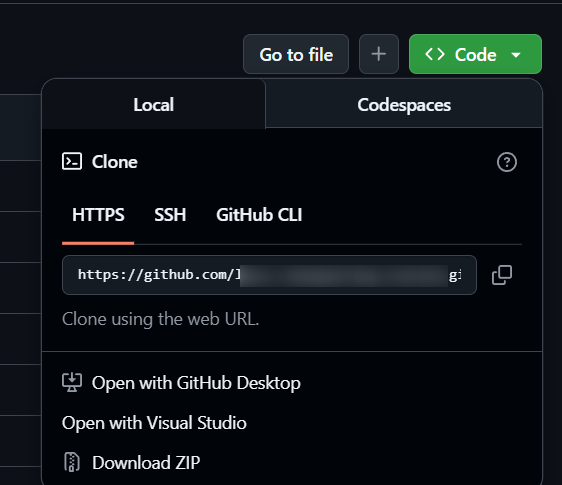
\includegraphics[width=0.5\textwidth]{images/example.png}
  \caption{GitHub 上的仓库页面}
  \label{fig:github-repo}
\end{figure}

接下来,我们需要将本地仓库与远程仓库关联。可以使用以下命令:
\begin{lstlisting}[language=bash]
git remote add origin <your-repo-url>
\end{lstlisting}
这将把远程仓库的 URL 添加为名为 origin 的远程仓库。origin 是习惯上的远程仓库名称。

现在我们要将这个本地仓库的代码推送到远程仓库中。可以使用以下命令:
\begin{lstlisting}[language=bash]
git push -u origin main
\end{lstlisting}
这里的 \texttt{-u} 选项表示将本地的 main 分支与远程的 main 分支关联起来,以后可以直接使用 \texttt{git push} 和 \texttt{git pull} 命令进行推送和拉取。

如果本地分支名称和远程有区别,(例如本地仓库主要分支是master,而远程仓库的主要分支是main),我们可以使用以下命令来推送代码:
\begin{lstlisting}[language=bash]
git push -u origin master:main
\end{lstlisting}
这将把本地的 master 分支推送到远程的 main 分支。

\subsubsection{使用仓库}

如果你是仓库的使用者,想要从远程仓库中拉取代码(但是本地没有这个仓库),可以使用以下命令:

\begin{lstlisting}[language=bash]
git clone <your-repo-url>
\end{lstlisting}

这样会在本地创建一个\textbf{新的}目录,并将远程仓库的代码克隆到该目录中。在克隆代码的时候,Git 会自动创建与远程同名的分支,并把它们与远程的 main 分支关联起来。

如果你已经有了本地仓库,并且想要将远程仓库的代码拉取到本地,经典的操作是以下命令:
\begin{lstlisting}[language=bash]
git pull origin main
\end{lstlisting}
直接使用 \texttt{git pull} 命令也是可以的,因为我们之前已经使用 \texttt{-u} 选项将本地分支与远程分支关联起来了。然而,需要注意的是现代的拉取操作往往不推荐使用 \texttt{git pull} 命令,因为它会自动合并远程分支的代码到本地分支,这可能会导致冲突。更推荐的做法是先使用 \texttt{git fetch} 命令拉取远程仓库的代码,然后再手动合并:
\begin{lstlisting}[language=bash]
git fetch origin
git merge origin/main
\end{lstlisting}
这样可以更好地控制合并过程,避免自动合并带来的问题。

如果你在本地做出了一些修改,想要将这些修改推送到远程仓库,可以使用以下命令:
\begin{lstlisting}[language=bash]
git push origin main
\end{lstlisting}
直接使用 \texttt{git push} 命令也可以。

如果存在某些提交在远程仓库中,而本地仓库没有这些提交,Git 会提示你先拉取远程仓库的代码,然后再推送本地的修改。这是因为 Git 不允许直接推送到远程仓库,除非本地仓库是最新的。如果你确定你不需要远程仓库的提交,可以使用以下命令强制推送本地的修改:
\begin{lstlisting}[language=bash]
git push -f origin main
\end{lstlisting}
但是请注意,这样会覆盖远程仓库的代码,可能会导致其他工作丢失,因此请谨慎使用。

\subsection{GitHub指南}

\subsubsection{这些都是什么东西?}

我们打开GitHub的一个仓库的时候,映入眼帘的类似这张图片内容。可以看到,这些图片中有很多不同的概念和功能。我们来逐一介绍一下。

\begin{figure}[!ht]
  \centering
  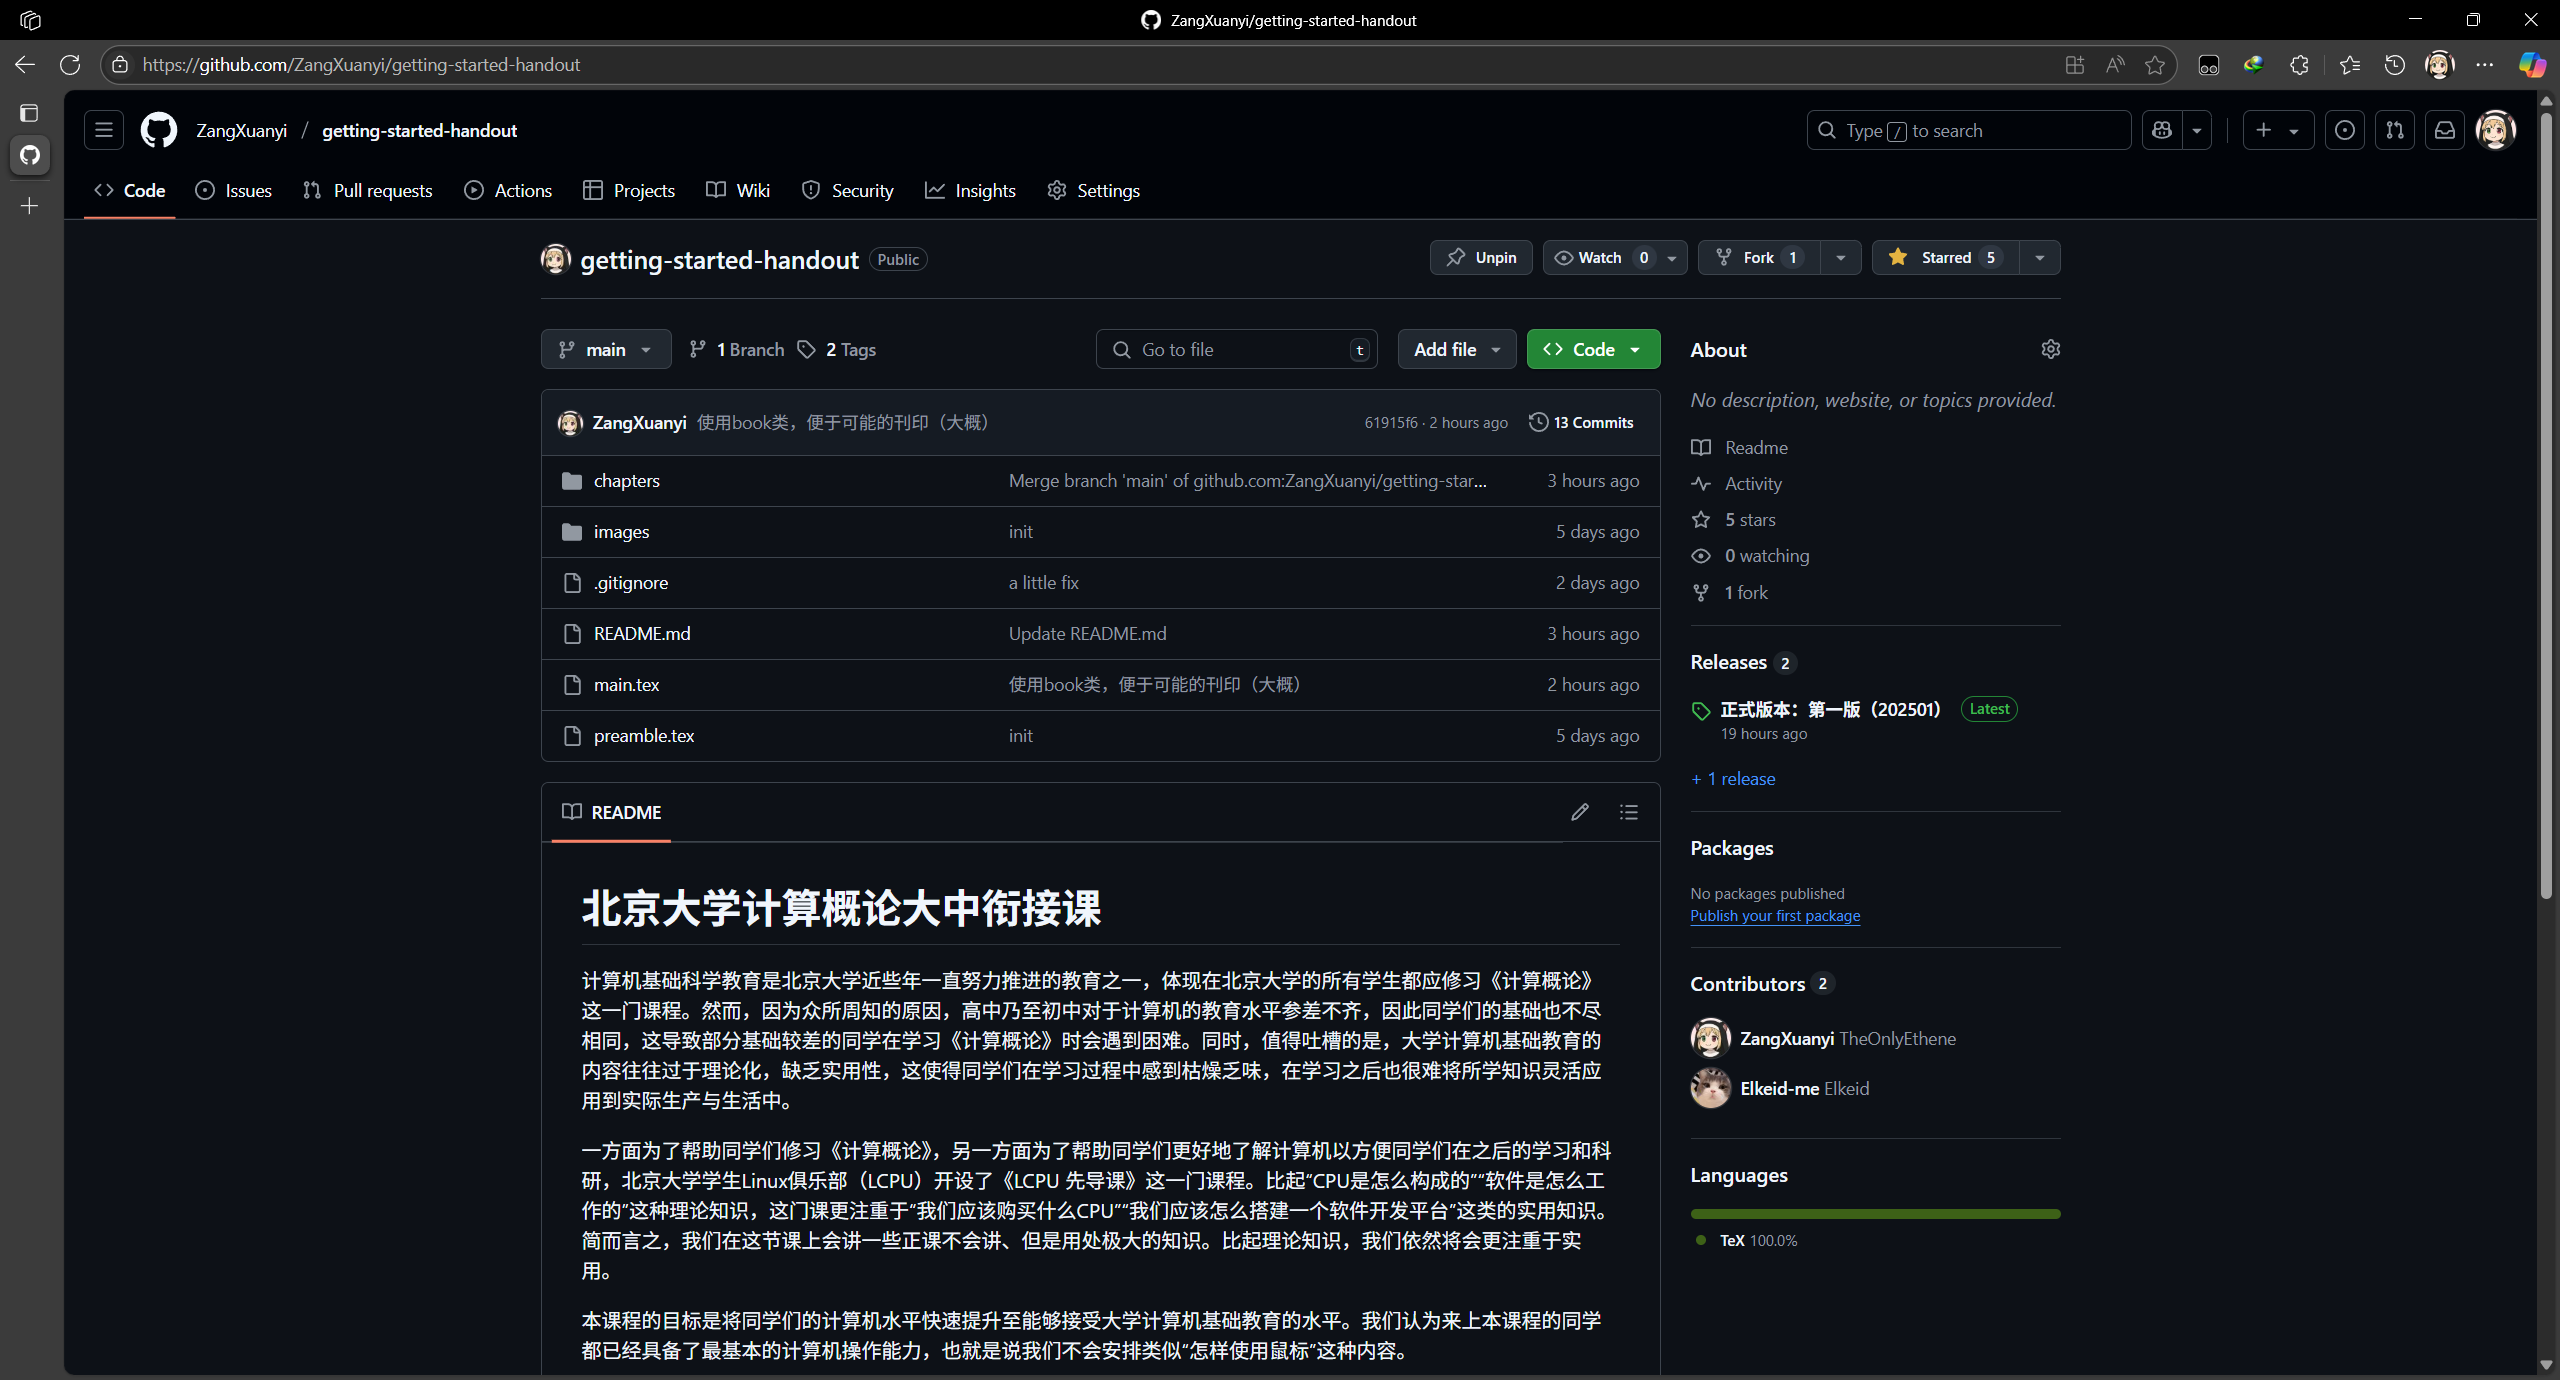
\includegraphics[width=\textwidth]{images/github.png}
  \caption{GitHub 仓库页面}
  \label{fig:github}
\end{figure}

在上面的一栏中,我们可以看到以code、issues、pull requests等为标题的选项卡。每个选项卡对应着一个功能模块。

\begin{itemize}
  \item \textbf{Code}:代码模块,显示仓库中的代码文件和目录结构。我们可以在这里浏览代码、下载代码、查看提交历史等。
  \item \textbf{Issues}:问题模块,用于跟踪和管理项目中的问题和任务。我们可以在这里创建新的问题、查看已有的问题、评论和解决问题等。在Gitea上,问题模块被称为“工单”(Tasks),这与它常用于公司自建库的特点有关。
  \item \textbf{Pull Requests}:合并请求模块,用于管理代码的合并和审查。我们可以在这里创建新的合并请求、查看已有的合并请求、评论和审查代码等。Pull Request(简称 PR)是 GitHub 和 GitLab 等平台提供的一种代码审查和合并的机制,具体内容可以参考\ref{sec:pull-request}节。
  \item \textbf{Actions}:自动化模块,用于管理项目的自动化工作流。我们可以在这里创建新的工作流、查看已有的工作流、运行和调试工作流等。
  \item \textbf{Projects}:项目模块,用于管理项目的进度和任务。我们可以在这里创建新的项目、查看已有的项目、添加任务和卡片等。
  \item \textbf{Wiki}:维基模块,用于管理项目的文档和知识库。我们可以在这里创建新的页面、编辑已有的页面、添加图片和链接等。GitHub Wiki 是 GitHub 提供的一种文档管理工具,可以帮助我们编写和维护项目的说明文档。
  \item \textbf{Security}:安全模块,用于管理项目的安全性和漏洞。我们可以在这里查看项目的安全报告、修复漏洞、配置安全策略等。
  \item \textbf{Insights}:洞察模块,用于分析项目的活动情况,例如提交历史、问题和合并请求的统计信息等。我们可以在这里查看项目的活跃度、贡献者的统计信息、代码的质量和覆盖率等。
  \item \textbf{Settings}:设置模块,用于管理项目的设置和配置。我们可以在这里修改项目的名称、描述、权限等属性。
\end{itemize}

靠下一行就是仓库的名称,右面是仓库的描述和一些操作按钮。Star 用来标记喜欢的仓库,Fork 用来复制仓库到自己的账户下,Watch 用来关注仓库的更新。

再靠下一行,我们可以看到仓库的分支(Branch)和提交(Commit)信息。分支是代码的不同版本,提交是代码的历史记录。我们可以在这里切换分支、查看提交历史、比较不同分支的差异等。同一行的那个绿色的Code按钮是用来下载代码的,可以选择下载为 ZIP 文件或者使用 Git 克隆仓库。我们非常推荐使用 Git 克隆仓库,因为这样可以更方便地管理代码和提交。

页面的左下方部分,在文件目录之下,是仓库的readme文件内容。README 文件是仓库的说明文档,通常包含项目的介绍、安装和使用说明、贡献指南等信息。我们可以在这里查看项目的详细信息。

页面右侧的一列是仓库的统计信息,包括提交历史、分支、标签、贡献者等。我们可以在这里查看项目的活跃度、贡献者的统计信息、代码的质量和覆盖率等。同时,我们也可以在这里找到仓库的发行版等信息。

\subsection{多人协作}

成熟的项目往往是由多人协作完成的,因此需要一些规范来管理代码的提交和合并等。GitHub、GitLab等提供了多种方式来支持多人协作,包括分支管理、代码审查、合并请求等。

\subsubsection{Fork}

Fork 是 GitHub 和 GitLab 等平台提供的一种代码复制和协作的机制。它允许用户将其他人的仓库复制到自己的账户下,从而可以在自己的仓库中进行修改和提交。这样可以使得修改更加方便(主要是防止权限不够),并且可以避免直接修改原仓库的代码。当然,权限足够的情况下,我们往往会直接在原仓库中创建新分支进行修改。

\subsubsection{Pull Request}\label{sec:pull-request}
Pull Request(简称 PR)是 GitHub 和 GitLab 等平台提供的一种代码审查和合并的机制。它允许开发者在完成某个功能或修复某个问题后,将自己的代码提交到主分支(通常是 main 或 master)之前,先进行代码审查和讨论。

PR 的工作流程通常如下:

\begin{enumerate}
  \item 开发者fork(分叉)一个仓库,或者在原仓库中创建一个新的分支。
  \item 开发者在自己的分支上进行开发,完成某个功能或修复某个问题。
  \item 创建一个PR,请求将自己的分支合并到主分支。PR 中可以包含对代码的描述、相关问题的链接等信息。
  \item 其他开发者可以对 PR 进行代码审查,提出修改意见或建议。
  \item 开发者根据审查意见修改代码,并更新 PR。
  \item 当 PR 获得足够的审查和批准后,可以将其合并到主分支。通常会有一个维护者或项目负责人来执行这个操作。
  \item 合并后,PR 会被关闭,相关的分支可以被删除;也可以保留,以便后续的开发和维护。
\end{enumerate}

\subsubsection{Lint}

在多人协作中,代码风格和规范的一致性非常重要。Lint 工具可以帮助我们检查代码中的潜在问题和不符合规范的地方。常见的 Lint 工具有 ESLint(用于 JavaScript)、Pylint(用于 Python)等。

如果我们在仓库中包含了 Lint 工具的配置文件(例如 .eslintrc.json 或 .pylintrc),那么在提交代码时,Git 会自动运行 Lint 工具,对代码进行检查。如果代码不符合规范,Lint 工具会给出相应的错误或警告信息。

Lint 工具通常会在 PR 中自动运行,并将检查结果反馈给开发者。开发者可以根据检查结果修改代码,确保代码符合项目的规范。

\subsubsection{成熟项目的分支管理策略}

在成熟的项目中,一般会采用一些分支管理策略来规范分支的使用和合并等。一般说来,同一个仓库中会有以下几种分支:(以下是Git Flow的工作管理策略)
\begin{itemize}
  \item main/master:主分支,通常是代码的稳定版本。一般禁止直接提交代码,只能通过合并其他分支来进行更改。
  \item develop/dev:开发分支,一般是集成了所有的新功能的基准分支,是开发的主要分支。该分支从main分出,最终也要进入main分支。对于一些较为轻量级的项目,有时候会直接使用feature分支来代替develop分支。
  \item feature/\textit{feature-name}:功能分支,每个新功能或改进都在独立的分支上进行开发。不同的开发者可以在不同的功能分支上工作,完成后再合并到develop分支。在功能完成开发后,通常会删除该分支。
  \item hotfix/\textit{hotfix-name}:热修复分支,一般是绕过开发流程,直接从main分支分出,修复完成后再合并回main分支和develop分支。热修复分支通常用于修复生产环境中的紧急问题,在问题彻底解决之后,该分支往往会被删除。
  \item release/\textit{release-name}:发布分支,一般用于准备发布新版本的代码。该分支从develop分出,经过测试和修复后再合并回main分支和develop分支。发布分支通常用于准备发布新版本的代码。在发布完成后,通常会删除该分支。不过现在往往会直接使用打标签的方式来替代发布分支。
\end{itemize}

开发的一般流程是:在main分支上发布了第一个稳定的版本后,会分出一个dev分支。之后,通常会禁止大多数人对main进行直接提交或者合并,所有新功能都在dev分支上开发,具体的形式是从dev分支上分出多个feature分支来进行多线、多功能的同时开发,且对于大型项目,dev分支往往也只允许合并,禁止小的提交。

有时候合并进dev分支的代码可能存在一些问题,而测试和检查又疏忽,导致合并进main分支之后出现了错误。此时,我们需要直接从main分支分出一个hotfix分支来修复问题,可能会采用一些临时的策略来修复问题。修复完成后,hotfix分支会被合并回main分支。在这之后,main分支会被合并进dev分支以同步代码,然后对hotfix分支上出现的问题加以更稳定的修复。在修复完成后,再将dev分支合并进main分支,此时可以删除hotfix分支。

除了Git Flow,还有其他一些分支管理策略,例如GitHub Flow、GitLab Flow等。GitHub Flow 是 GitHub 提出的分支管理策略,主要用于快速迭代和持续集成,其开发非常轻量级,一般只有 main/master 和 feature 分支。GitLab Flow 则是 GitLab 提出的分支管理策略,多出了产品分支和预发布分支等,分别用于生产环境和预发布环境。

\section{密钥进阶}

在初阶课程中,我们已经知道了密钥是什么东西,并且知道了在大多数的情况下要使用密钥而不是密码来进行身份验证。但是关于“怎么使用和管理”密钥,则没有进行详细介绍。在本节中,我将会详细地介绍密钥的使用和管理。

\subsection{SSH密钥的生成}

在Windows上,我们需要安装系统功能OpenSSH Client来进行密钥的初步使用。在Linux和Mac上,OpenSSH通常是预装的。如果没有安装,请自行查找相关资料进行安装。

在安装完成后,我们可以使用以下命令来生成密钥对:
\begin{lstlisting}[language=bash]
ssh-keygen -t rsa -b 4096 -C "<你的邮箱地址>"
\end{lstlisting}

上述命令会生成一个 RSA 密钥对,密钥长度为 4096 位,并且会在密钥中添加一个注释(通常是你的邮箱地址)。执行该命令后,会提示你输入密钥的保存路径和密码。默认情况下,密钥对会保存在 \texttt{\textasciitilde/.ssh/id\_rsa} 和 \texttt{\textasciitilde/.ssh/id\_rsa.pub} 中。

RSA密钥对是最常用的密钥对之一,不过因为 RSA 密钥对的安全性已经不如以前了,因此现在推荐使用 Ed25519 密钥对。可以使用以下命令生成 Ed25519 密钥对:
\begin{lstlisting}[language=bash]
ssh-keygen -t ed25519 -C "<你的邮箱地址>"
\end{lstlisting}

生成密钥对后,我们需要将公钥(\texttt{id\_rsa.pub} 或 \texttt{id\_ed25519.pub})添加到远程服务器或服务(例如 GitHub、GitLab、CLab 等)的 SSH 密钥列表中。我们可以使用任何喜欢的编辑器打开上述公钥文件,复制其中的内容,并将其粘贴到指定的位置。\textbf{\color{red}同时,私钥(\texttt{id\_rsa} 或 \texttt{id\_ed25519})必须保密,绝对不能泄露给任何人!}

如果我们本地是Linux或者Mac且能够直接访问远程服务器,可以使用以下命令将公钥复制到远程服务器上:
\begin{lstlisting}[language=bash]
ssh-copy-id user@remote-server
\end{lstlisting}

我们也可以手动将公钥复制到远程服务器的 \texttt{\textasciitilde/.ssh/authorized\_keys} 文件中。我们可以使用记事本或者code等编辑器打开公钥文件,复制其中的内容,然后在远程服务器上使用以下命令将其添加到 \texttt{\textasciitilde/.ssh/authorized\_keys} 文件中。以上方法适用于无法使用 ssh-copy-id 命令的情况,例如Windows系统。

为了保护私钥的安全,我们可以为私钥设置一个密码。这样,在使用私钥进行身份验证时,需要输入密码才能解锁私钥。可以在生成密钥对时设置密码,也可以在后续使用 \texttt{ssh-keygen} 命令修改密码。

设置密码的方式非常简单。在生成密钥对时,系统会提示你输入密码。如果你不想设置密码,可以直接按 Enter 键跳过。

如果你已经生成了密钥对,但没有设置密码,可以使用以下命令为私钥设置密码:
\begin{lstlisting}[language=bash]
ssh-keygen -p -f ~/.ssh/id_rsa
\end{lstlisting}

实际上如果保密需求不是非常高的话,我们可以不设置密码。因为使用密钥除了安全性以外,最大的好处是可以免去每次连接远程服务器时输入密码的麻烦。而如果设置了密码,则每次连接远程服务器时都需要输入密码,这样就失去了使用密钥的便利性。

\subsection{密钥的使用}

在生成密钥对并将公钥添加到远程服务器或服务后,我们就可以使用密钥进行身份验证了。使用密钥进行身份验证的方式与使用密码类似,只不过需要指定私钥文件。

\subsubsection{连接到远程服务器}

可以使用以下命令连接到远程服务器:
\begin{lstlisting}[language=bash]
ssh -i ~/.ssh/id_rsa user@remote-server
\end{lstlisting}
如果你使用的是 Ed25519 密钥对,则需要将 \texttt{id\_rsa} 替换为 \texttt{id\_ed25519}。

如果你已经将私钥添加到 SSH Agent(实际上这确实是更一般的情况)中,可以直接使用以下命令连接到远程服务器:
\begin{lstlisting}[language=bash]
ssh user@remote-server
\end{lstlisting}

\subsubsection{Git托管}

GitHub的有两种托管代码的方式:HTTPS 和 SSH。HTTPS 是通过用户名和密码进行身份验证,而 SSH 是通过密钥进行身份验证。我们建议使用 SSH 进行身份验证,因为它更加安全和方便,且无需忍受网络代理的折磨。

我们需要将公钥添加到 GitHub 的 SSH 密钥列表中。可以在 GitHub 的设置页面中找到 SSH 密钥列表,然后点击“添加 SSH 密钥”按钮,将公钥粘贴到文本框中。

如果你使用的是 Windows 系统,可能需要将公钥转换为 OpenSSH 格式。可以使用以下命令将公钥转换为 OpenSSH 格式:
\begin{lstlisting}[language=bash]
ssh-keygen -i -f ~/.ssh/id_rsa.pub
\end{lstlisting}

添加公钥后,我们就可以使用 SSH 进行身份验证了。在某些情况下,我们可能需要手动指定使用的哪一个密钥文件。可以使用以下命令将 SSH 密钥添加到 SSH Agent 中:
\begin{lstlisting}[language=bash]
ssh-add ~/.ssh/id_rsa
\end{lstlisting}

这样可以免去每次连接远程服务器时指定密钥文件的麻烦。

\subsection{使用VS Code建立SSH连接}

除了使用终端建立SSH连接到远程服务器以外,还可以使用一些其他的工具来建立SSH连接。这时候我们还要请出那位大神:VS Code(怎么哪都有你)。

VS Code 提供了一个名为 Remote-SSH 的扩展,可以帮助我们通过 SSH 连接到远程服务器,并在远程服务器上进行开发。这样,可以在SSH连接中使用一个很方便的图形化界面,以进行和Windows相似的便捷操作。

安装 Remote-SSH 扩展后,我们可以在 VS Code 的界面找到远程连接的选项,一般是左下角的蓝色按钮,图标类似这个$\lessgtr$数学符号。点击这个按钮后,会弹出一个菜单,点选“连接到主机”选项,会让你输入\texttt{user\@ host}类似的远程服务器地址。输入完成后,如果是一个新的远程服务器,Code会让你把它加入到已知主机列表中,用户可以视情况添加到系统配置文件或者其他的配置文件中。

然后,Code会弹出一个新的窗口,试图连接到远程服务器,可能会要求你输入远程服务器的密码和系统类型等信息。连接完成后,就可以在远程服务器上进行开发了。此时,Code会在左侧的资源管理器中显示远程服务器的文件系统(当然你需要打开一个文件夹)。

在Code中,如果不是用终端而是用Code的图形界面来打开新的文件夹,那么每一次打开文件夹都会重新进行一次身份验证。如果你使用的是密码,则需要反复输入,非常麻烦。这时我们一定要尽可能地使用密钥进行登录。

\section{Windows的文件管理和自动化操作}\label{sec:windows-file-management}

在计算机上,我们经常需要对文件进行管理和自动化操作。文件管理包括文件的增删改查、移动复制等操作,而自动化操作则是通过脚本或工具来实现对文件的批量处理和自动化任务。

本段将以Windows为例,介绍一些常用的文件管理和自动化操作的相关知识。有关Linux文件系统的相关知识将会在下一章节介绍。

\subsection{文件系统基础知识}

文件系统是操作系统用来管理存储设备上数据的结构和方法。它定义了如何在存储设备上组织、存储和访问文件和目录。文件系统的主要功能包括文件的增删改查等操作。

对于一个文件而言,文件系统会为其分配一个唯一的标识符(通常是文件名),并将其存储在一个目录结构中。为了方便理解,我们可以将文件系统理解成一个巨大的档案馆,每个文件就像是档案馆中的一份档案,目录则有些像书架、文件夹等存储档案的工具或者设备,而目录结构则是档案馆中的分类系统。

对于任何文件或者目录,都有一个唯一的路径(Path)来标识它在文件系统中的位置。路径是由目录和文件名组成的字符串,通常使用斜杠(/)或反斜杠(\textbackslash)作为分隔符。在Windows系统下的一个路径示例是:\texttt{D:\textbackslash dir\textbackslash file.txt}。这种从盘符(根)开始的路径结构叫做\textbf{绝对路径}。

在有些时候,使用绝对路径并不合适。同样以档案举例子,假设某档案要求参阅同一档案袋里的某一份其他档案。这时我们如果使用绝对路径记录的话,需要记录整个档案的路径,例如“辽宁-张三-身份证”依赖于“辽宁-张三-出生证明”。现在张三移居北京,这个档案袋也整体移到北京。如果张三的身份证依赖的出生证明路径依然是“辽宁-张三-出生证明”,这时就会找不到这个东西了。

为了解决这一问题,我们引入了\textbf{相对路径}的概念。相对路径是相对于当前目录的路径,不需要从根目录开始。例如,如果当前文件是 \texttt{D:\textbackslash dir\textbackslash file.txt},那么文件 \texttt{D:\textbackslash dir\textbackslash file2.txt} 的相对路径就是 \texttt{file2.txt},而文件 \texttt{D:\textbackslash dir\textbackslash dir1 \textbackslash file3.txt} 的相对路径就是 \texttt{dir1\textbackslash file3.txt}。

在一些比较严谨的文档中,你也可以看到相对路径的写法是 \texttt{./file2.txt} ,其中 \texttt{./} 表示当前目录。这在命令行中常用,尤其是在使用命令行执行可执行文件的时候只能这样写,防止你误执行了系统目录下的同名文件。

在Python中,你甚至可以看到相对路径的写法是 \texttt{.file2},其中 \texttt{.} 表示当前目录。这种写法在某些情况下也可以使用,但是大多数时候这个点(.)开头的文件指的是隐藏文件,我们不推荐在除了Python之外的场合使用这种写法。

有时候相对路径需要跨目录访问,这需要“向上一级”操作。在这种情况下,我们可以使用两个点(..)来表示上一级目录。例如,如果当前文件是 \texttt{D:\textbackslash dir\textbackslash file.txt},那么文件 \texttt{D:\textbackslash dir2\textbackslash file4.txt} 的相对路径就是 \texttt{..\textbackslash dir2\textbackslash file4.txt}。

\subsection{Windows的文件系统结构}

Windows使用的是NTFS文件系统,基于驱动器(Drive),每个驱动器都有一个盘符(例如C:、D:等)。每个驱动器既可以是一个物理存储设备,也可以是一个存储设备的某一分区(主分区或者逻辑分区)。Windows的文件系统结构是树形结构,每个驱动器下都有一个根目录(例如C:\textbackslash),根目录下可以有多个子目录和文件。

在Windows下,路径使用反斜杠(\textbackslash)作为分隔符。例如\texttt{D:\textbackslash dir\textbackslash file.txt}。尽管如此,Windows也支持使用正斜杠(/)作为分隔符,两者也可以混合使用。不过我们建议在Windows下使用反斜杠(\textbackslash)作为分隔符,以保持一致性。

Windows中有如下一些常用的文件夹:
\begin{itemize}
  \item \texttt{C:\textbackslash Windows}:Windows操作系统的核心文件夹,包含系统文件和驱动程序。
  \item \texttt{C:\textbackslash Program Files}:安装的应用程序的默认文件夹,通常包含64位应用程序。
  \item \texttt{C:\textbackslash Program Files (x86)}:安装的32位应用程序的默认文件夹。
  \item \texttt{C:\textbackslash Users}:用户文件夹,包含每个用户的个人文件和设置。
  \item \texttt{C:\textbackslash Downloads}:下载文件夹,默认存储从互联网下载的文件。
\end{itemize}

\subsection{文件的默认打开方式}

在Windows中,每种文件类型都有一个默认的打开方式。当我们双击一个文件时,系统会根据文件的扩展名(例如.txt、.jpg等)来确定使用哪个应用程序打开该文件。

一般情况下,除非你知道你在干什么,否则不要随便修改文件的默认打开方式。但是部分软件会改变文件的默认打开方式,例如安装了某个文本编辑器后,可能会将所有的文本文件(.txt)默认打开方式改为该编辑器。

我们非常建议同学们在安装软件时,仔细阅读安装向导中的选项,避免不必要的修改;同时,尽可能不要安装多个同类软件,以免造成文件默认打开方式的混乱。

\subsection{高效整理与搜索文件}

在Windows中,我们可以使用文件资源管理器(File Explorer)来浏览和管理文件。文件资源管理器提供了多种视图模式(例如列表视图、详细信息视图等),可以帮助我们更高效地浏览和整理文件。

我们可以使用右键菜单来对文件进行各种操作,例如复制、移动、重命名、删除等。除此之外,在文件夹菜单下可以找到排序方式、分组方式等选项,可以帮助我们更高效地整理文件。

我们在整理文件的时候,要遵循一定的命名规范。例如,文件名应该简洁明了,能够清楚地表达文件的内容;文件夹名应该具有层次性,能够清晰地表示文件的分类和组织结构。同时,由于各种各样的兼容原因,文件和文件夹名中不要包含特殊字符,并且尽量避免使用空格。

\subsection{搜索工具}

在Windows上,我们可以使用文件资源管理器的搜索功能来查找文件。只需要在文件资源管理器的搜索框中输入关键词,系统就会自动搜索当前文件夹及其子文件夹中的文件。这个搜索的问题是速度非常缓慢,尤其是在文件数量较多的情况下(例如全盘搜索)。

如果我们需要更高级的搜索功能,可以使用第三方搜索工具,例如 Everything、Listary 等。这些工具可以提供更快、更准确的搜索结果,并且支持多种搜索条件和过滤器。

\subsection{自动化脚本}

\subsubsection{批量处理文件示例}

一般情况下,整理相机里的照片时,我们会将照片按照日期和地点等信息进行分类。但是如果照片数量过多,手动逐个重命名会非常繁琐。此时,我们可以使用自动化脚本来批量处理文件。

在Windows上,我们可以使用批处理脚本(Batch Script)或 PowerShell 脚本来实现自动化操作。批处理脚本是一种简单的脚本语言,可以通过编写一系列命令来实现对文件的批量处理。不过PowerShell脚本很多新手并不熟悉,批处理脚本风格又太老,因此我们推荐使用Python的\texttt{os}库来实现自动化操作。

一个典型的示例是:

\begin{lstlisting}[language=python]
import os
for filename in os.listdir("."):
    if filename.endswith(".jpg"):
        os.rename(filename, "pic_" + filename)
\end{lstlisting}

使用以上脚本,我们可以将当前目录下所有的 .jpg 文件批量重命名为 pic\_ + 原文件名的形式。对以上代码进行相关修改,则可以进行其他的批量处理操作,例如移动文件、删除文件、批量添加前后缀、按照规则排序等。

如果不想保留原文件名,而是使用“照片 (1)”这样的格式,就不必写脚本了。可以直接使用Windows的批量重命名功能。只需要选中所有的照片,右键点击,选择“重命名”,然后输入新的文件名(例如“照片”),系统会自动将所有选中的照片重命名为“照片 (1)”、“照片 (2)”等格式。

\subsubsection{定时自动备份脚本示例}

我们可以使用Python 的\texttt{shutil}库来实现定时自动备份脚本。以下是一个简单的示例:
\begin{lstlisting}[language=python]
import shutil
import datetime

# 备份文件夹到指定位置
backup_dir = f"backup_{datetime.date.today()}"
shutil.copytree("我的文档", backup_dir)
\end{lstlisting}

以上脚本会将“我的文档”文件夹备份到当前目录下,并以“backup\_YYYY-MM-DD”的格式命名备份文件夹。我们可以将该脚本设置为定时任务,定期自动执行备份操作。

\subsubsection{更进阶的自动化}

在Windows中,我们可以使用任务计划程序(Task Scheduler)来设置定时任务。任务计划程序允许我们创建和管理定时任务,可以设置任务的触发条件、执行时间等。

要创建一个定时任务,可以按照以下步骤操作:
\begin{enumerate}
  \item 打开任务计划程序(可以在开始菜单中搜索“任务计划程序”)。
  \item 点击“创建基本任务”。
  \item 输入任务的名称和描述。
  \item 设置触发条件,例如每天、每周等。
  \item 设置操作,例如运行脚本或程序。
  \item 完成设置,保存任务。
\end{enumerate}

通过任务计划程序和自动化脚本,我们可以实现定时自动备份、定时清理临时文件等自动化操作。

\subsubsection{跨设备同步}

在现代的工作环境中,我们经常需要在多台设备之间同步文件。Windows 提供了多种方式来实现跨设备同步,例如使用 OneDrive、Google Drive 等云存储服务。当然,以上云存储服务需要支付一定的费用才能获得更多的存储空间。

作为替代,我们可以使用SyncThing等开源工具来实现跨设备同步。SyncThing 是一个分布式的文件同步工具,可以在多台设备之间自动同步文件,而无需依赖云存储服务。

\end{document}